% !TEX encoding = UTF-8
% !TEX program = pdflatex
% !TEX root = InformationRetrieval.tex
% !TEX spellcheck = it-IT

% 18 Novembre 2016
%\chapter{Valutazione dei sistemi di reperimento}
%\section Il paradigma Cranfield
\FloatBarrier
\section{Recall}

Il richiamo misura quanti documenti rilevanti sono stati recuperati, rispetto la totalità dei documenti rilevanti presenti all'interno del pool. Anche in questo caso si tratta di un valore compreso tra 0 e 1, dove 1 indica la run perfetta.

\begin{figure}[htbp]
	\centering
	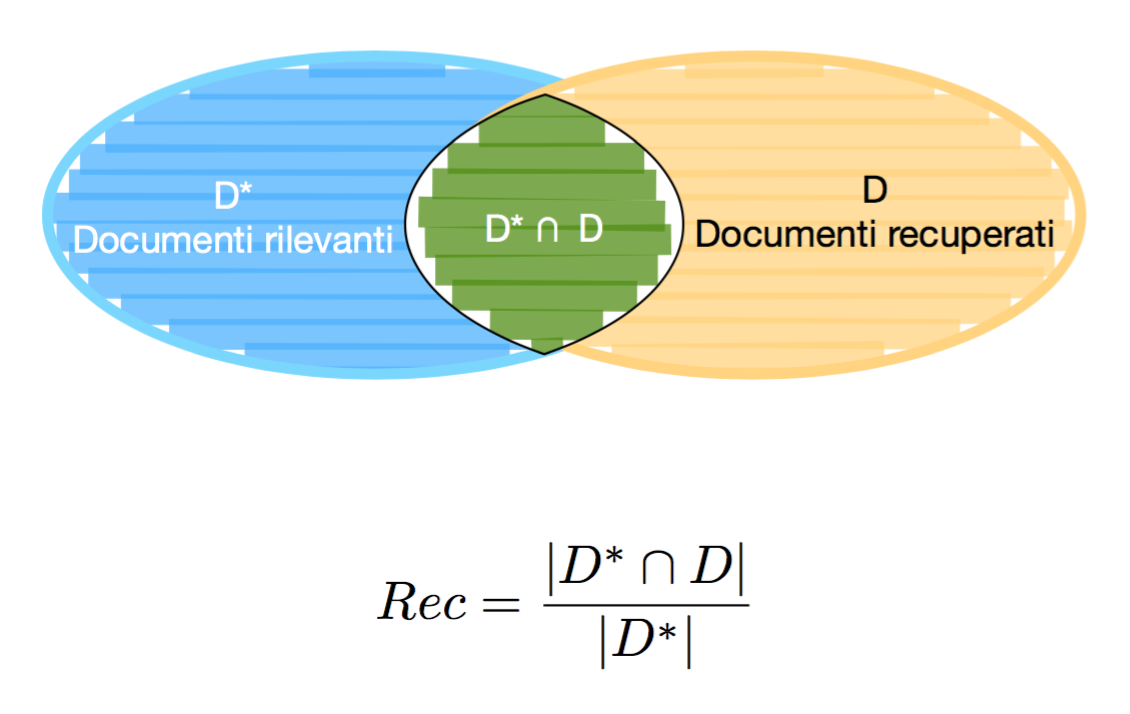
\includegraphics[width=0.6\textwidth]{images/l15-fig-1.png}
\end{figure}

Il valore $|D^*|$ rappresenta il numero di documenti rilevanti per il topic presenti nel pool e viene anche chiamato \textbf{recall base} per un determinato topic. Si tratta di un valore fisso che dipende dal topic e viene determinato analizzando il pool.

Più formalmente, sia $D$ un insieme finito di documenti, $T$ un insieme finito di topic, $GT$ la ground truth definita su $D$ e $T$ e $REL$ un insieme totalmente ordinato di giudizi di rilevanza. La \textbf{recall base} è definita come:

\begin{align*}
	RB : T &\to \mathbb{N} \\
		t &\to RB_t = \Big| \big\{ d \in D \ | \ GT(t,d) \succ \min(REL) \big\} \Big|
\end{align*}

\noindent Ovvero come la cardinalità dell'insieme dei documenti $D$ che per il topic $t$ hanno un giudizio di rilevanza maggiore del minimo, dove il minimo giudizio di rilevanza è quello associato ad un documento non rilevante.
La recall base è un riferimento importante per l'analisi delle prestazione di un sistema IR, perché per essere perfetto un sistema deve recuperare tutti i documenti rilevanti, ordinati per giudizio di rilevanza decrescente.

\begin{figure}[htbp]
	\centering
	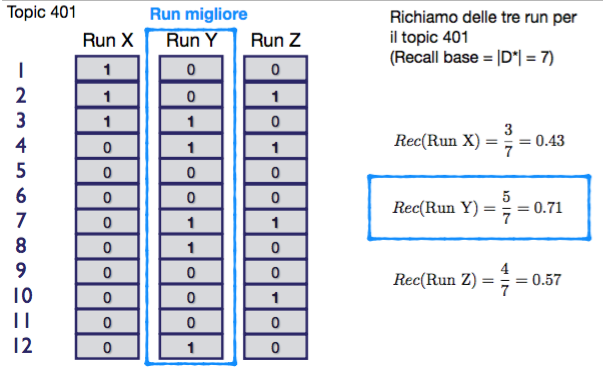
\includegraphics[width=0.7\textwidth]{images/l15-fig-2.png}
	\caption{Esempio di calcolo della recall.}
\end{figure}

\textbf{{\color{Red} Possibile domanda:}} Si definisca il concetto di recall base.
\FloatBarrier
\section{E-Measure e F-measure}

\`E utile avere un numero unico per esprimere la qualità della run e che riesca a combinare la precisione e il richiamo

\begin{figure}[htbp]
	\centering
	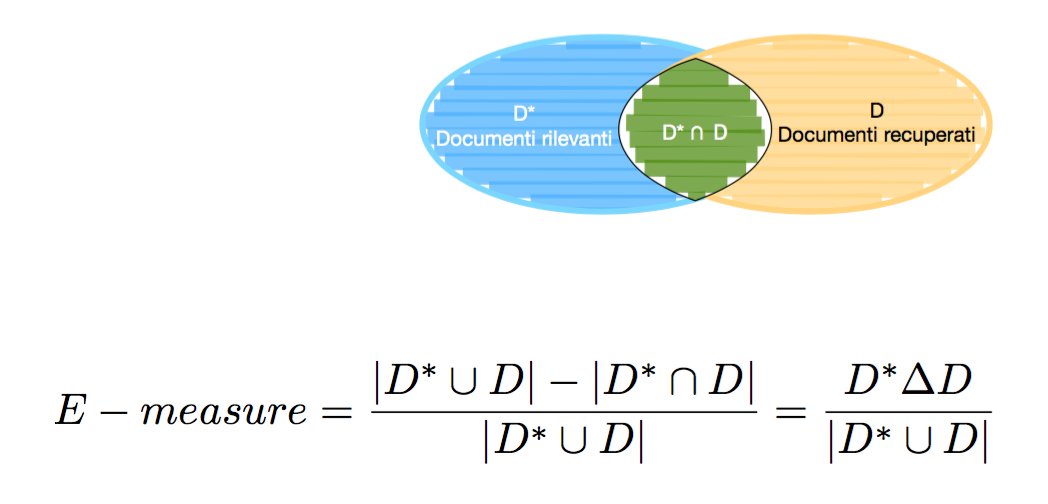
\includegraphics[width=0.7\textwidth]{images/l15-fig-3.png}
\end{figure}

Se l'intersezione è vuota, ottengo un \textit{E-measure} uguale a 1, che è il caso di retrieval pessimo.
Se invece l'\textit{E-measure} è 0, i due insiemi coincidono e quindi il retrieval è perfetto.

Siccome questa misura è contro-intuitiva si è scelto di utilizzare

$$
F\text{-}measure = 1 - E\text{-}measure
$$

Tuttavia, anche questa misura, come precision e recall, non è una misura ranked, perché non viene preso in considerazione l'ordine.
\FloatBarrier
\section{Precisione e richiamo con cut-off}

Per alcuni task di ricerca è importante tenere in considerazione l'ordine dei risultati e quindi è utile avere delle misure che tengano conto anche di questo.

L'idea quindi è quella di calcolare la precisione solamente sui primi $k$ elementi recuperati. Questa nuova misura prende il nome di $perc@k$.

$$
prec@k = \frac{1}{k}\sum\limits_{j=1}^{k} \mathbf{\tilde{r}}_t[j]
$$

Un caso particolare è quello di $p[RB_t] = prec@RB_t$ che è la precision con cut-off dato dalla dimensione della recall base per un dato topic. Questa misura prende anche il nome di \textbf{R-Prec}.

\begin{figure}[htbp]
	\centering
	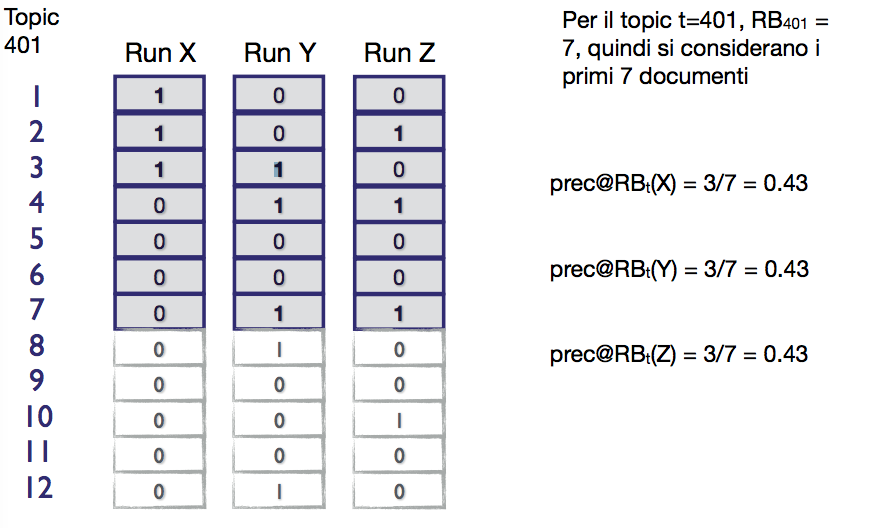
\includegraphics[width=0.6\textwidth]{images/l15-fig-3-1.png}
	\caption{Esempio di calcolo della R-Prec per il topic $t = 401$ con $RB_{401} = 7$.}
\end{figure}

\textbf{{\color{Red} Possibile domanda:}} Si definiscano le misure di Precisione a cut-off 10 e precisione alla recall base. Se ne descrivano le principali differenze.

Lo stesso ragionamento può essere effettuato per il richiamo:

$$
recall@k = \frac{1}{RB_t} \sum\limits_{j=1}^{k} \mathbf{\tilde{r}}_t[j]
$$

\FloatBarrier
\section{Curva Richiamo-Precisione}

Questa curva calcola la precisione in funzione di $x$ punti di richiamo, in modo da poter disegnare una curva con i punti di richiamo sull'asse delle ascisse e la precisione sulle ordinate.

\begin{figure}[htbp]
	\centering
	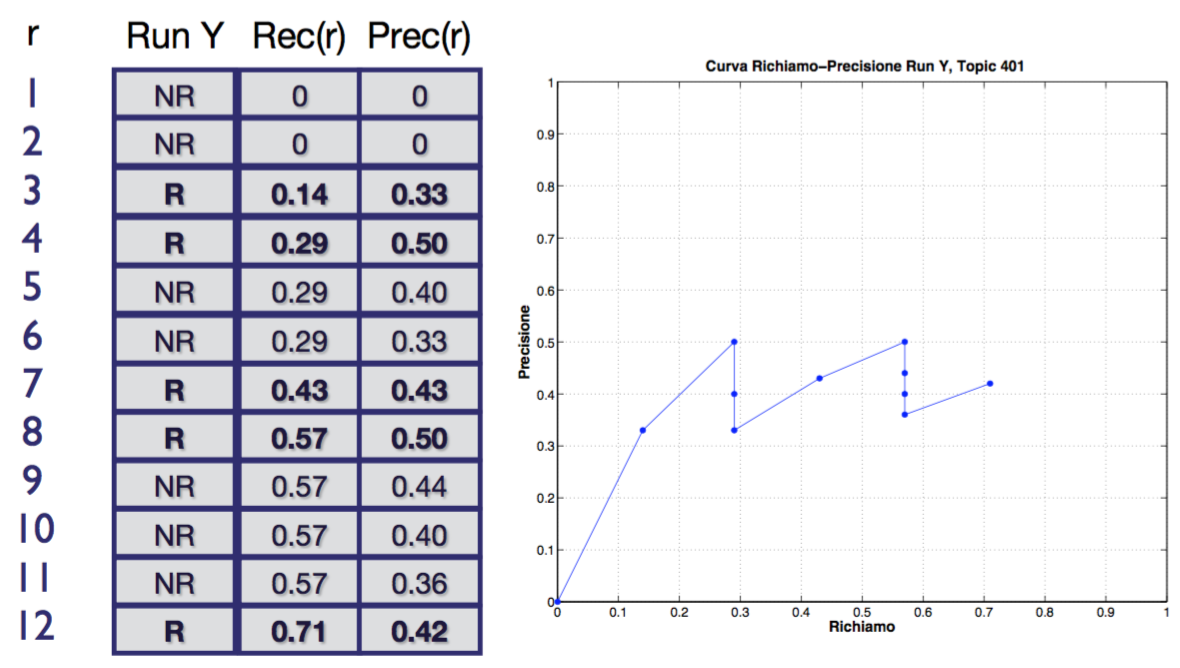
\includegraphics[width=0.65\textwidth]{images/l15-fig-4.png}
	\caption{Esempio della curva richiamo-precisione.}
\end{figure}

Ovvero per ogni livello di rango vengono calcolate la precisione e il richiamo con cut-off a quel livello.
Quindi per il primo livello di rango viene calcolata la \textit{recall} come se la run avesse lunghezza 1 e la precisione come $prec@1$, per il secondo la recall considera solo i primi due documenti e la precisione è $prec@2$ e così via fino a raggiungere il rango massimo che equivale alla lunghezza della run.

Questa curva però ha un sacco di problemi, perché intanto non è una funzione, inoltre non è possibile utilizzarla per comparare due run distinte. C'è poi anche da tenere in considerazione che uno stesso sistema può produrre run diverse.

Una variante è la curva \textbf{interpolata}: una curva simile che viene ottenuta considerando 11 punti fissi di richiamo (\textbf{11-point recall-precision}).

Come prima cosa viene definito un set di punti che rappresentano dei livelli di richiamo:

$$
RP = \{ 0, 0.1, 0.2, \ldots 1 \}
$$

\noindent dopodiché viene calcolato per ogni punto $rp \in RP$ la \textbf{precisione interpolata a \textit{rp}}:

$$
IP_{rp} = \max_{1 \leq r \leq N | Rec(r) \geq rp} Prec(r)
$$

\noindent ovvero ad ognuno dei punti dell'insieme $rp$ viene associato il più alto valore di precisione ottenuto sui primi $r$ valori della run che hanno un richiamo maggiore del punto.

Quindi nel lato pratico:

\begin{enumerate}
	\item Per ogni livello di rango $r$ della run calcolo $rec@r$ e $prec@r$
	\item Per ogni punto $rp$ calcolo $IP_{rp}$ come il \textbf{massimo} valore di $prec@r$ tale che $rec@r > rp$
\end{enumerate}

\begin{figure}[htbp]
	\centering
	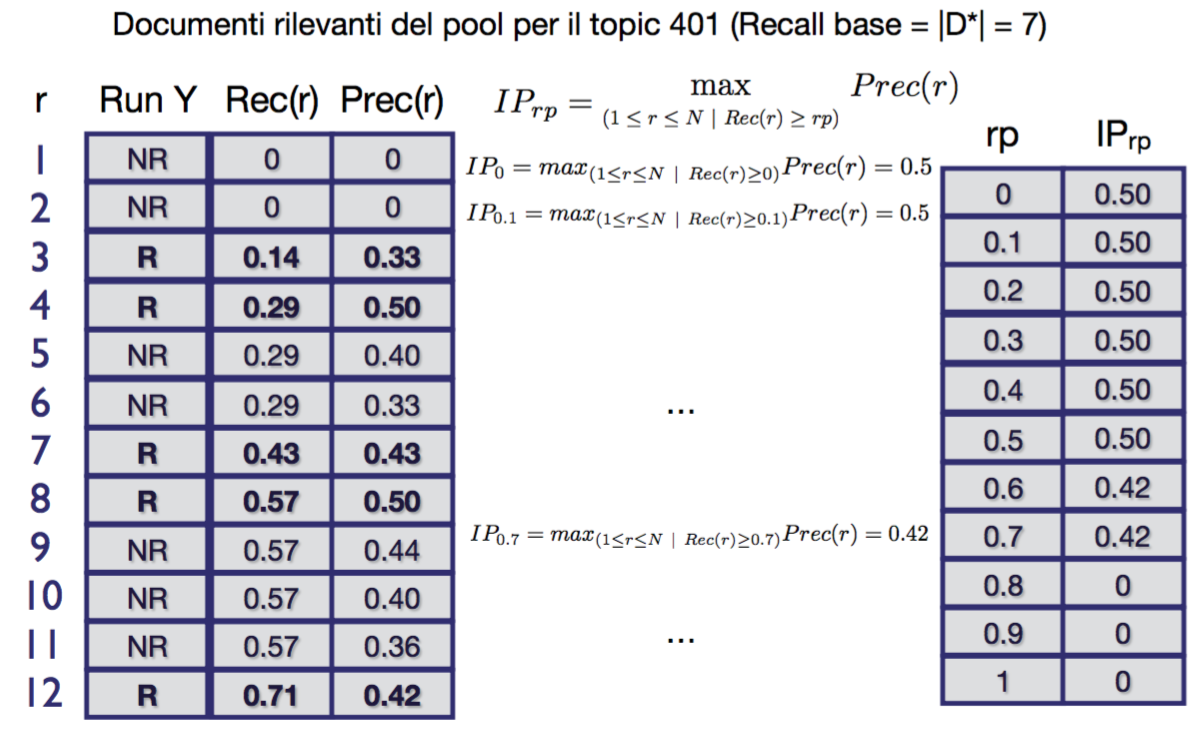
\includegraphics[width=0.8\textwidth]{images/l15-fig-5.png}
	\caption{Esempio di calcolo della curva richiamo-precisione interpolata.}
\end{figure}

\begin{figure}[htbp]
	\centering
	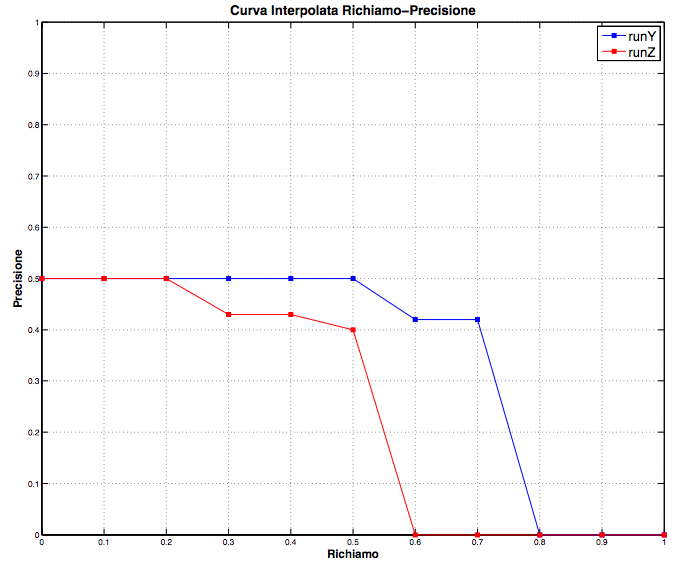
\includegraphics[width=0.6\textwidth]{images/l15-fig-6.png}
	\caption{Esempio di curva richiamo-precisione interpolata.}
\end{figure}

\FloatBarrier
\section{11-Point Average Precision}

La curva richiamo precisione va bene per giudicare ad occhio quale delle due curve va meglio, però si può fare di più utilizzando l'11-\textbf{Point Average Precision} che effettua la media di tutti i valori di precisione interpolata calcolati.

$$
\text{11pt-AP} = \frac{\sum_{rp\in\{0,0.1,\ldots \ 1 \}}IP_{rp}}{11}
$$

C'è però un'effetto indesiderato perché la precisione a valori alti di richiamo ha lo stesso peso di quelli a livelli bassi, mentre si vorrebbe dare maggiore peso alla precisione ai livelli più alti di rank, ovvero sui primi documenti della run.
Tipicamente si usa quindi l'\textbf{Average Precision}.

Dato un topic $t \in T$, una recall base $RB_t$, $REL =\{ nr, r \}$ e una run $\mathbf{r}_t$ di lunghezza $N$ tale che:

$$
\forall i \in [1, N], \tilde{\mathbf{r}}_t = \begin{cases}
0 \quad &\text{se } \hat{\mathbf{r}}_t[i] = nr \\
1 \quad &\text{se } \hat{\mathbf{r}}_t[i] = r \\
\end{cases}
$$

\noindent l'average precision è definita come:

$$
AP = \frac{1}{RB_t}\sum\limits_{k=1}^{N} \underbrace{\tilde{\mathbf{r}}_t[k]}_{\text{relevance weight dell'elemento \textit{k}}} \overbrace{\frac{\sum\limits_{h=1}^{k} \tilde{\mathbf{r}}_t[h]}{k}}^{prec@k}
$$

Le misure di questo tipo prendo il nome di \textbf{top heavy} perché danno più peso ai documenti rilevanti in posizioni alte del rank.

\begin{figure}[htbp]
	\centering
	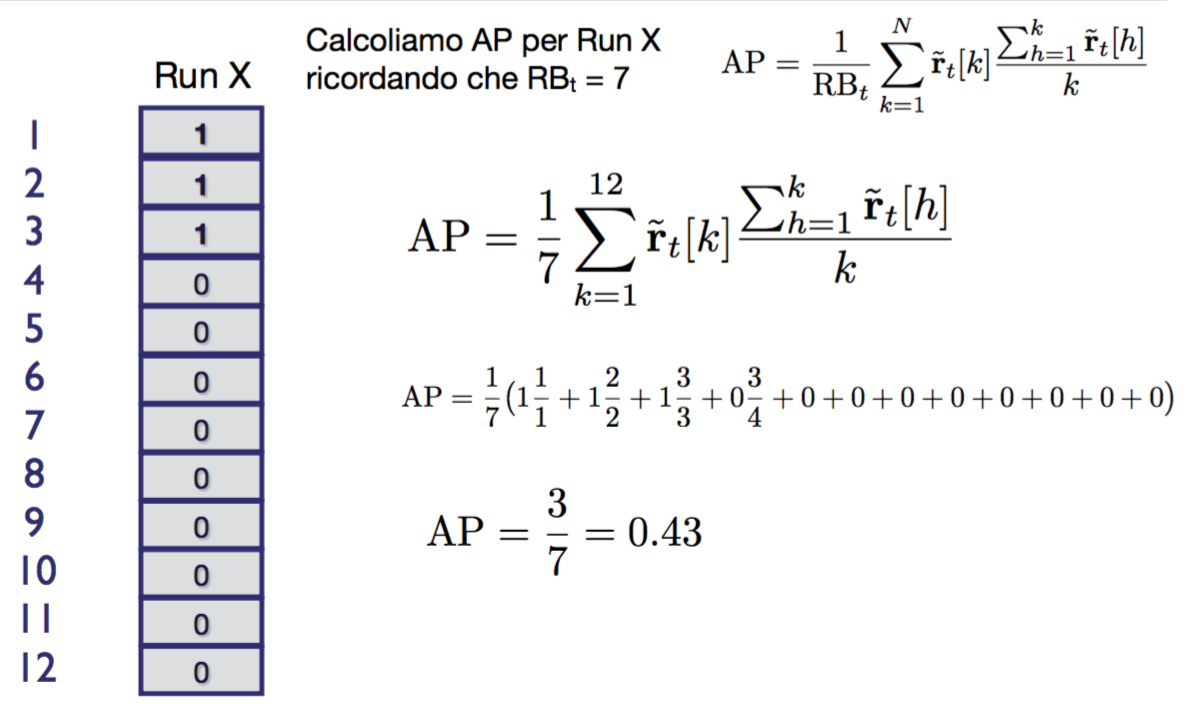
\includegraphics[width=0.7\textwidth]{images/l15-fig-7.png}
	\caption{Esempio di calcolo di Average Precision.}
\end{figure}

\textbf{{\color{Red} Possibile domanda:}} Si definiscano le misure 11pt-AP e AP e si descrivano i principali vantaggi e svantaggi delle due misure in termine di efficacia.

\section{Valutazione di un sistema su più topic}

Le misure viste finora valutano la singola run su un topic, ma tipicamente le campagne di valutazione sono fatte su 50 o 100 topic.

L'idea base è quella di fare la media aritmetica delle run sui singoli topic. Si parla quindi di \textbf{Mean Average Precision} (\textbf{MAP}). Detta anche la \textit{media media precisione}.

$$
MAP(R) = \frac{\sum_{t\in T}AP(\mathbf{r}_t)}{|T|}
$$

Tipicamente è una brutta idea fare la media di una misura che dipende dalla recall base, perché la dimensione della recall base varia di topic in topic. 
Ma nel campo di valutazione dell'IR, AP è una misura che piace e quindi si fa comunque la media. 

Quindi va bene utilizzare la \textbf{MAP} ma non va bene fare la media delle precisioni alla recall-base (\textbf{R-prec-media}).
